\section{Cơ sở thiết kế trò chơi}
\subsection{Tổng quan trò chơi}
\hspace*{1cm} \textbf{MeowSQL Knight} là một trò chơi nhập vai Phiêu lưu chiến đấu theo lượt. Thay vì sử dụng các thao tác thông thường bằng các nút, người chơi tương tác bằng các nhập câu truy vấn và thực thi chúng, thu thập dữ kiện để chiếm lấy ưu thế trong chiến đấu, đánh bại quái vật và hoàn thành màn chơi.\\
\begin{figure}[H]
	\centering
	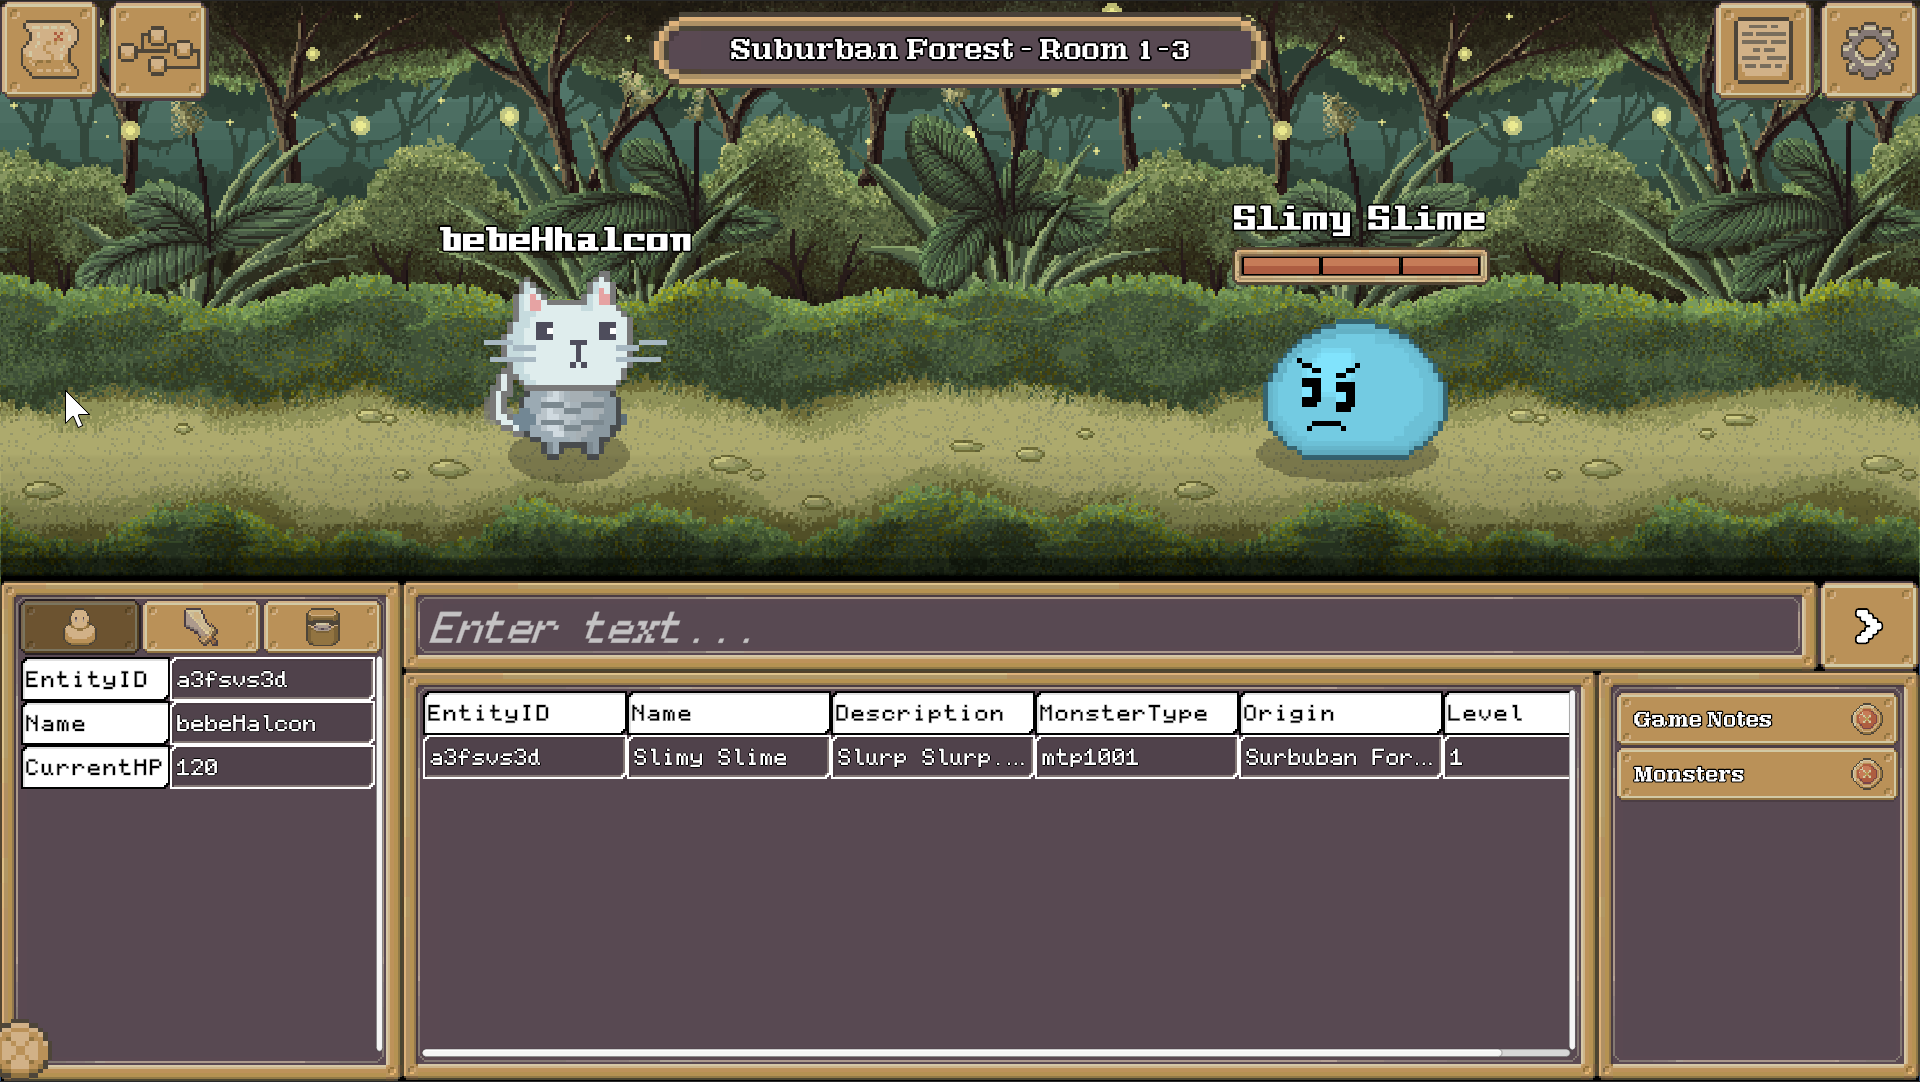
\includegraphics[width=\textwidth]{Images/Overall.png}
	\vspace{0.5cm}
	\caption{Tổng quan một màn chơi trong MeowSQL Knight}
\end{figure}
\hspace*{1cm} Người chơi sẽ sử dụng các câu truy vấn để khai thác schema cho sẵn. Sử dụng \textbf{select} để hiện nội dung các record lên màn hình, thu thập thông tin từ những dữ liệu đó. Ngoài ra cũng có thể \textbf{insert} và \textbf{delete} những record trên bảng và xem phản ứng của trò chơi sẽ như thế nào. Người chơi sẽ tấn công quái vật bằng các vũ khí mà người chơi mang vào trận chiến, tuy nhiên không thể tấn công quái vật một cách đơn thuần, người chơi sẽ phải tấn công vào các điểm yếu của quái vật nằm trên các bộ phận khác nhau. Để tương tác với game (tấn công quái vật, dùng vật phẩm), người chơi sẽ insert các tham số vào các bảng có chức năng đặc biệt, sau khi chèn xong thì hành động sẽ được thực thi.\\
\hspace*{1cm} Trong Schema này, các thực thể như người chơi, quái vật, bộ phận chí mạng của quái vật,... đều sử dụng chung ID có cấu trúc như nhau. Để tiêu diệt quái vật, người chơi phải nhắm đến các bộ phận chí mạng này, cũng như xác định được ID của chúng để có thể tấn công chính xác, bằng không các đòn đánh của người chơi sẽ bị trượt.\\
\hspace*{1cm} Người chơi phải tìm cách khai thác schema một cách hiệu quả trong chiến đấu. Đi kèm với việc lựa chọn trang bị hợp lý và tận dụng lợi thế môi trường, giành chiến thắng, hoàn thành màn chơi và đi sâu hơn để tìm ra bí ẩn của trò chơi.


\subsection{Sơ lược cốt truyện}
\hspace*{1cm} Trong một thế giới game RPG có chủ đề là động vật bình thường, bạn là một kỵ sĩ mèo đang đi rừng để tìm nguyên liệu, mọi thứ diễn ra một cách bình thường. \\
\hspace*{1cm} Đột nhiên, trò chơi bỗng hoạt động không đúng so với trước kia, các quái vật trở nên hung hãn hơn, nguy hiểm hơn, lẽ ra chỉ cần đánh bằng các phương pháp thông thường đã có thể diệt sạch chúng, nhưng kì lạ thay, các phương pháp thông thường không còn có hiệu quả với chúng nữa. Đám quái vật vùng lên làm loạn cả thế giới game, khiến thế giới game bị lỗi nghiêm trọng, và nếu cứ tiếp tục như vậy, trò chơi sẽ không thể chơi được nữa.\\
\hspace*{1cm} Chính lúc này, nhân vật chính của chúng ta bị một con slime bao vây, lẽ ra 1 nhát từ kiếm của cậu có thể hạ gục con Slime, tuy nhiên, trong thế giới game bị rối loạn như thế này là không thể. Cậu cứ đánh trong vô vọng, trong khi con quái vật giận dữ tiến gần định nuốt chửng cậu. Đột nhiên, một tia sáng xuất hiện giết chết con quái vật đó. Là Nhà phát triển (Dev) của trò chơi này. Anh ấy đã kiểm tra hệ thống thế giới game và phát hiện ra bạn là một trong những object hiếm hoi còn sống trong thế giới game này. Để hỗ trợ bạn, Dev cấp cho bạn 1 năng lực lớn: bạn có thể xem schema của game và thực hiện các câu truy vấn SQL để khai thác schema và chiến đấu. Vì chỉ có sử dụng SQL mới có thể đánh bại các quái vật SQL. \\
\hspace*{1cm} Dev muốn đặt niềm tin vào bạn vì Dev không thể khởi dộng lại Project game này, nó là một project chạy trên server nhưng cậu đã mất quyền kiểm soát cả server và project. Dev muốn bạn đi sâu vào bên trong lõi của game và tìm ra lý do khiến game trở nên như vậy. Bạn là hy vọng của thế giới game này, và là hy vọng của cả Dev. Bạn bắt đầu đi vào sâu trong thế giới, mang sứ mệnh vô cùng cao cả, không chỉ để cứu thế giới này.

\subsection{So Sánh các sản phẩm tương tự trên thị trường}
\subsubsection{Game 1}
\subsubsection{Game 2}
\subsubsection{Điểm khác biệt của ...}

\subsection{Luật chơi}
\hspace*{1cm} Mỗi màn chơi, người chơi sẽ được đưa đến một bản đồ, gồm các phòng liên thông với nhau. Nhiệm vụ của người chơi là sử dụng các câu truy vấn để tương tác nhân vật chính, hoàn thành yêu cầu được đưa ra trong mỗi căn phòng, đến điểm cuối của bản đồ và hoàn thành màn chơi.

\subsubsection{Bản đồ trong màn chơi}

\subsubsection{Chiến đấu}


\subsubsection{Win condition}
\subsubsection{Lose condition}

\subsection{Các đối tượng chính trong màn chơi}